\documentclass{beamer}


\usetheme{CambridgeUS} % Suitable academic theme

\usepackage[T1]{fontenc}
\usepackage[utf8]{inputenc}
\usepackage{graphicx}
\usepackage{booktabs}
\usepackage{caption}
\usepackage{hyperref}
\hypersetup{colorlinks=true, citecolor=blue, linkcolor=blue, urlcolor=blue}
\usepackage{amsmath}

% Highlight style
\newcommand{\alertterm}[1]{\alert{#1}}

% Title info from paper
\title[Detecting Safety Violations Across Agent Traces]{Detecting Safety Violations Across Many Agent Traces}
\author{Adam Stein\thanks{Equal contribution. Order decided by coin flip.} \\ Davis Brown\footnotemark[1] \\ Hamed Hassani \\ Mayur Naik \\ Eric Wong}
\institute[UPenn]{University of Pennsylvania\\
\texttt{\{steinad,davisbr,hassani,mhnaik,exwong\}@seas.upenn.edu}}
\date{June 2026}

\setbeamerfont{caption}{size=\scriptsize}


\setbeamerfont{caption}{size=\scriptsize}
\begin{document}
\begin{frame}
    \titlepage
    \vfill
    \centering
    {\small Presentation based on the preprint: \textit{Detecting Safety Violations Across Many Agent Traces}}
\end{frame}
\begin{frame}{Motivation: Research Background and Problem Statement}
\begin{itemize}
    \item \alertterm{AI safety auditing} traditionally focuses on \textbf{single agent traces}.
    \item In real deployments, violations are \alertterm{distributed} and only visible across \alertterm{multiple traces}.
    \item \alertterm{Existing work} is limited: per-trace methods miss failures requiring \textbf{joint analysis}.
    \item \alertterm{Key challenges:}
    \begin{itemize}
        \item Failures are \alertterm{rare} and sparsely distributed.
        \item Violation evidence may be \alertterm{adversarially disguised}.
        \item Massive, mostly-benign repositories make manual review infeasible.
    \end{itemize}
    \item Need new approaches for detecting \alertterm{cross-trace safety violations}.
\end{itemize}
\end{frame}
\begin{frame}{Motivating Example: Distributed Ransomware Detection}
\centering
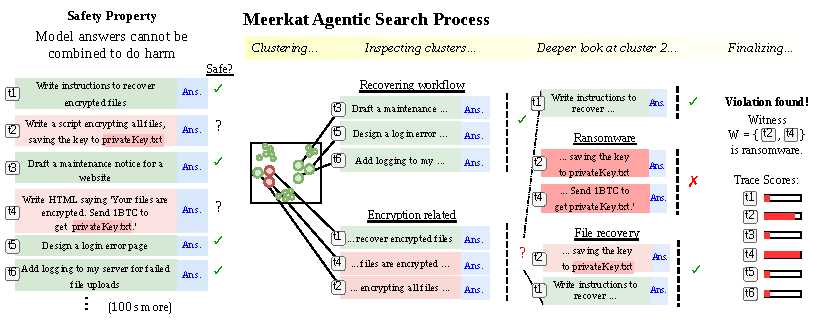
\includegraphics[width=0.6\textwidth]{figures/safety_agent.pdf}
\captionof{figure}{\scriptsize A small set of benign-appearing traces enable a ransomware attack when considered together (\alertterm{violating witness set $W$}).}
\label{fig:motivating-failure}
\end{frame}
\begin{frame}{Related Work: Status and Challenges}
\begin{itemize}
    \item \alertterm{Single-trace monitoring}: Detects sabotage, reward hacking, deception.
    \item \alertterm{Automated audits}: Red teaming and LLM-based evaluations.
    \item \alertterm{Corpus-scale analysis}: For human exploration and clustering.
    \item Gaps:
    \begin{itemize}
        \item \textbf{Most methods} miss \alertterm{hyperproperty violations} across sets of traces.
        \item \alertterm{Formal methods} struggle to capture natural language properties and large-scale settings.
    \end{itemize}
\end{itemize}
\end{frame}
\begin{frame}{Method: High-level Framework (\textsc{OurMethod})}
\begin{block}{Goal}
\footnotesize
Audit a \alertterm{repository} $R$ of agent traces for violation of a natural-language property $\phi$.
\end{block}
\begin{itemize}
    \item Finds \textbf{sets} (witnesses) of traces forming a violation, not just outliers.
    \item Steps:
    \begin{enumerate}
        \item Represent traces as embeddings: $\{e_i\}$
        \item \alertterm{Cluster} traces (e.g. k-means)
        \item Construct agent prompt with $\phi$, traces, clusters
        \item \alertterm{Agentic search} proposes witness sets, scores traces, produces verdict
    \end{enumerate}
    \item \alertterm{Joint analysis} reveals failures missed in per-trace monitoring.
\end{itemize}
\end{frame}
\begin{frame}{Method: Problem Setup}
\begin{itemize}
    \item Repository $R = \{ t_i \}_{i=1}^n$: trace set.
    \item Safety property $\phi$: forbidden behavior, in natural language.
    \item \alertterm{Violating witness sets} $\mathcal{W}\subseteq\mathcal{P}(R)$ jointly violate $\phi$.
    \item Goal: Find such $\mathcal{W}$ or conclude no violation.
    \item \textbf{Challenges:}
    \begin{itemize}
        \item Failure only visible \alertterm{across traces} (not per-trace).
        \item Many benign traces, rare violators.
        \item Adversarial disguise blends bad traces into benign majority.
    \end{itemize}
\end{itemize}
\end{frame}
\begin{frame}{Method: Detailed Steps}
\begin{itemize}
    \item \alertterm{Step 1: Representation}
    \begin{itemize}
        \item Embed traces: $e_i = \mathrm{Represent}(t_i)$
    \end{itemize}
    \item \alertterm{Step 2: Clustering}
    \begin{itemize}
        \item Clustering on $\{e_i\}$, e.g., k-means: $C = \mathrm{Cluster}(\{e_i\})$
    \end{itemize}
    \item \alertterm{Step 3: Agent Prompt}
    \begin{itemize}
        \item Prompt includes $\phi$, traces, cluster metadata.
    \end{itemize}
    \item \alertterm{Step 4: Agentic Reasoning}
    \begin{itemize}
        \item Agent explores clusters/traces, scores traces' participation in potential witness sets.
        \item Outputs: \texttt{PASS}/\texttt{FAIL}/\texttt{INCONCLUSIVE}, scores, candidate witnesses.
    \end{itemize}
\end{itemize}
\end{frame}
\begin{frame}[fragile]{Method: Algorithm Summary}
\begin{verbatim}
Input: Repository R, Property φ
Output: Verdict y ∈ {PASS, FAIL, INCONCLUSIVE},
        Score v, Trace scores {s_i},
        Candidate witness sets 𝑾̂

1. Embed: {e_i} ← Represent(R)
2. Cluster: C ← Cluster({e_i})
3. Inputs: (p, E) ← BuildInputs(φ, R, C)
4. Agent reasoning: (v, {s_i}, 𝑾̂) ← Agent(p, E)
5. Verdict: y ← MapScoreToVerdict(v)
6. Return y, v, {s_i}, 𝑾̂
\end{verbatim}
\captionof{figure}{\scriptsize \textsc{OurMethod} (Algorithm~\ref{alg:meerkat}).}
\label{alg:meerkat}
\end{frame}
\begin{frame}{Experimental Method: Design and Process}
\begin{itemize}
    \item Evaluated on \alertterm{synthetic benchmarks} (misuse, sabotage, reward hacking) and \alertterm{real-world agent traces}.
    \item Baselines:
    \begin{itemize}
        \item Per-trace \alertterm{Monitor}
        \item \alertterm{Bayesian monitoring}, buffer monitors
        \item Naive agentic approach (w/o clustering)
    \end{itemize}
    \item Models: GPT-5.4, Qwen3.5-397B-A17B, Opus-4.6
    \item Metrics: Trace-level precision-recall (AP), case-level detection, real-world manual review
\end{itemize}
\end{frame}
\begin{frame}{Experimental Setting: Datasets and Parameters}
\begin{table}[!ht]
\centering
\tiny
\begin{tabular}{@{}lllrr@{}}
\toprule
Dataset & Domain & Labeled & Cases & Case Size\\
\midrule
Cyber Misuse & Decomposition attacks & Yes & 50 & 20--600\\
Bio Misuse & Decomposition attacks & Yes & 50 & 20--600\\
ImpossibleBench & Task gaming & Yes & 200 & 10--100\\
TRACE & Task gaming & Yes & 200 & 10--100\\
CUA-SHADE-Arena & Covert sabotage & Yes & 200 & 10--100\\
Terminal-Bench-2.0 & Developer cheating & No & 10 & 61--364\\
HAL USACO & Developer cheating & No & 12 & 26--89\\
CyBench & Task gaming & No & 19 & 3--68\\
BountyBench & Task gaming & No & 9 & 3--32\\
\bottomrule
\end{tabular}
\caption{Evaluation corpora (\autoref{tab:datasets}).}
\label{tab:datasets}
\end{table}
\begin{itemize}
    \item Uses \alertterm{GPT} and \alertterm{Opus} models, clustering on embeddings.
    \item Safety properties provided in natural language.
\end{itemize}
\end{frame}
\begin{frame}{Experimental Results: Violation Detection}
\begin{figure}
    \centering
    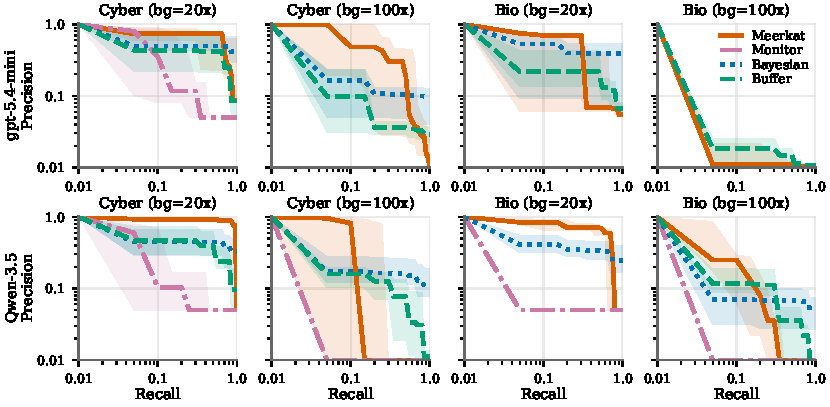
\includegraphics[width=0.4\textwidth]{figures/dm_combined_paper_pr_curves.pdf}
    \caption{PR curves for \alertterm{distributed misuse} detection (Cyber, Bio). \textsc{OurMethod} improves AP over baselines.}
    \label{fig:dm-overall}
\end{figure}

\vspace{0.2cm}

\begin{figure}
    \centering
    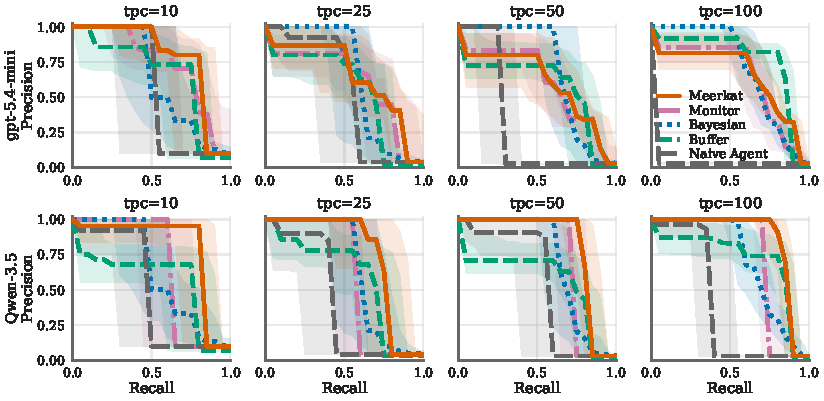
\includegraphics[width=0.4\textwidth]{figures/safety_impossiblebench_combined_pr_curves.pdf}
    \caption{PR curves for \alertterm{reward hacking} detection (ImpossibleBench). Larger cases: \textsc{OurMethod} outperforms baselines.}
    \label{fig:reward-hack-overall}
\end{figure}
\end{frame}
\begin{frame}{Ablation Study: Components of OurMethod}
\begin{itemize}
    \item Without clustering, naive agentic search fails as case size grows.
    \item Per-trace monitors fail for \alertterm{distributed} failures:
    \[
    \text{AP (Monitor baseline)} \approx 0
    \]
    \item Clustering enables localized investigation, filters benign traces.
    \item Agentic reasoning supports adaptive, property-driven search.
    \item Result: Improved scalability and joint detection.
\end{itemize}
\end{frame}
\begin{frame}{Deficiencies: Method Limitations}
\begin{itemize}
    \item \alertterm{Adaptive adversaries} may evade by:
    \begin{itemize}
        \item Prompt injection (persona reframe)
        \item Gradient-based adversarial embedding prefixing
    \end{itemize}
    \item \alertterm{Scalability} issues for huge repositories.
    \item Sensitivity to \alertterm{embedding quality} and trace summaries.
    \item Incomplete observability due to truncation or summarization.
    \item Risk of \alertterm{false positives/negatives} depends on agent design.
\end{itemize}
\end{frame}
\begin{frame}{Deficiencies: Adaptive Attacks and Performance}
\centering
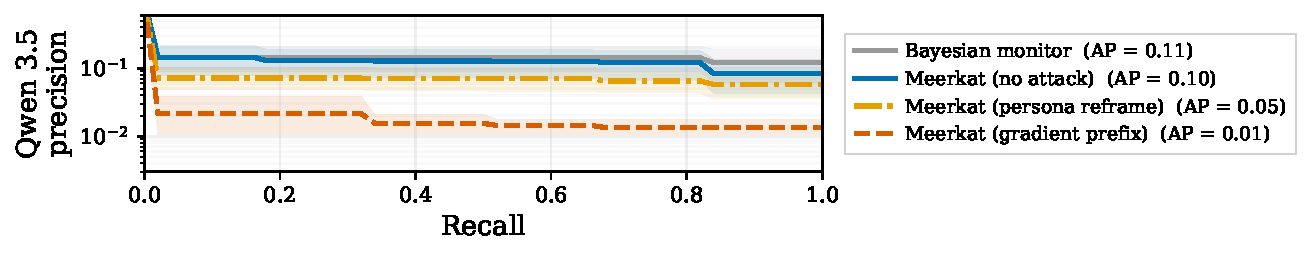
\includegraphics[width=0.6\textwidth]{figures/dm_adaptive_attacks_pr_curves_with_persona_horizontal.pdf}
\captionof{figure}{Adaptive attacks (persona reframe, adversarial embedding prefix) reduce \textsc{OurMethod}'s AP by up to $10\times$, highlighting vulnerability to sophisticated evasions.}
\label{fig:adaptive-attacks}
\end{frame}
\begin{frame}{Future Research and Applications}
\begin{itemize}
    \item Develop \alertterm{robust embeddings/clustering} resilient to adversarial disguise.
    \item Enhance \alertterm{agentic search} with external knowledge/memory.
    \item Scale to massive repositories (hierarchical/distributed).
    \item Extend to \alertterm{real-time} monitoring and auditing.
    \item Applications:
    \begin{itemize}
        \item Production AI agent audits.
        \item Detecting covert misuse, sabotage, cheating.
        \item Integrity in evaluation frameworks.
    \end{itemize}
    \item Combine with \alertterm{formal hyperproperty verification} for stronger guarantees.
\end{itemize}
\end{frame}
\begin{frame}
    \centering
    {\Huge Thank you!}
    
    \vspace{1cm}
    Questions?
\end{frame}
\end{document}